\documentclass[handout]{beamer}
% \documentclass{beamer}
\usepackage{color}
\usepackage{amsmath}
\usepackage{amssymb}
\usepackage{amsfonts}
\usepackage[utf8x]{inputenc}
\usepackage{longtable}
\usepackage{pdfpages}
\usetheme{MPIM}
\logo{}
% \mode<handout|presentation>{
\newcount\mylineno
\mylineno=0
\def\tblnewline{%
  \global\advance\mylineno by 1
  \ifnum\mylineno=7
    \global\mylineno=0
    \\
    \pagebreak
  \else
    \\
  \fi
}
% }
% \mode<article>{
% \newcount\mylineno
% \mylineno=0
% \def\tblnewline{%
%   \global\advance\mylineno by 1
%   \ifnum\mylineno=7
%     \global\mylineno=0
%     \\
%     \pagebreak
%   \else
%     \\
%   \fi
% }
% }
\newcommand{\derr}[2]{\frac{\partial #1}{\partial #2}}
\newcommand{\fav}[1]{\widetilde{#1}}
\newcommand{\xav}[1]{\left\langle{#1}\right\rangle}
\newcommand{\tav}[1]{\overline{#1}}
\newcommand{\source}[2]{\ensuremath{\mathcal{S}_{#1}^{\mathrm{#2}}}}
\newcommand{\force}[2]{\ensuremath{\mathcal{F}_{#1}^{\mathrm{#2}}}}
\newcommand{\mr}[1]{\ensuremath{\mathrm{\ #1}}}
\newcommand{\sgse}{e}
\newcommand{\rese}{E}
\newcommand{\code}[1]{{\tt #1}}
\newenvironment{codenv}{\tt}{}

\usepackage{pgfpages}
\usepackage{textcomp}
% \mode<handout>\pgfpagesuselayout{4 on 1}[a4paper,border shrink=5mm,landscape]
\title[UCLALES Tutorial]{Using the UCLA Large Eddy Simulation code }
\author[HERZ-CC]{Thijs Heus, Bjorn Stevens, Axel Seifert, Cathy Hohenegger}
\institute{Max Planck Institute for Meteorology}
\date{November 7 - 11, 2011}

\begin{document}
\begin{frame}[plain]
\titlepage
\end{frame}


\subtitle{UCLALES Tutorial}
 
\author{Thijs Heus}
\lecture{Overview of UCLA LES}{overview}
\begin{frame}{This Week}
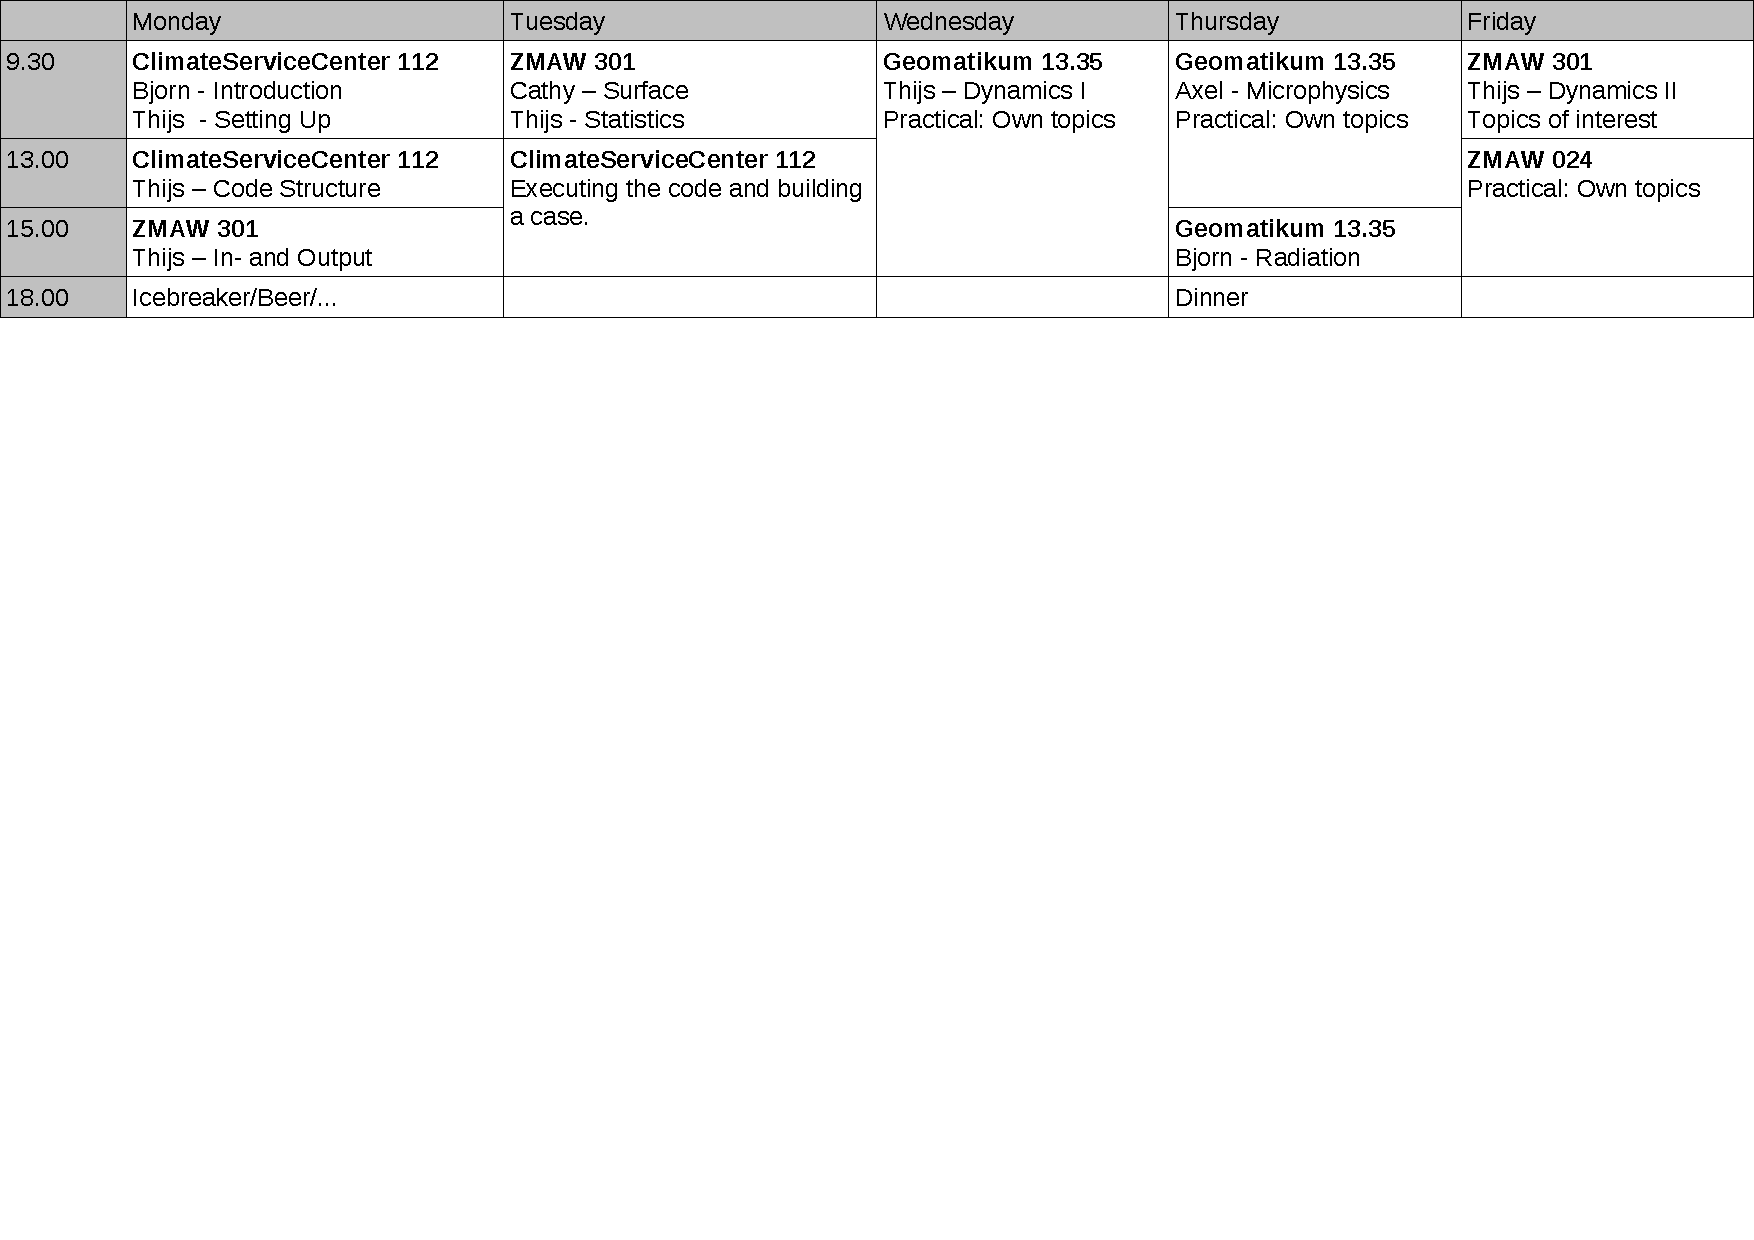
\includegraphics[width=\textwidth]{schedule.pdf}
\end{frame}
\begin{frame}{Our Group}
 \begin{itemize}
  \item Hans-Ertel Zentrum for research on Clouds and Convection
  \item Led by Cathy Hohenegger and Axel Seifert
  \item Funded by Deutscher Wetter Dienst
  \item Hunt for knowledge on convective clouds in various conditions
  \item Large Eddy Simulations are our primary (but not only) tool
 \end{itemize}

\end{frame}

\begin{frame}[<+->]{Cascade of Models}
 \begin{itemize}
  \item General Circulation Models
  \item Regional Models
  \item \alert{Large-Eddy Simulations}
  \item Direct Numerical Simulations
 \end{itemize}

\end{frame}
\begin{frame}[<+->]{Cascade of Models}
\framesubtitle{General Circulation Models}
\begin{itemize}
 \item Domain size: Entire Earth
 \item Horizontal Boundary conditions: None
 \item Horizontal grid spacing: $50 \mathrm{km}$
 \item Total number of points: about $400 \times 400 \times 100 $
 \item Simulation duration: Weeks - millennia
 \item Resolved: Hadley Circulation, fronts, ...
 \item Parameterized: Clouds,  Boundary layers, Surface, Microphysics
\end{itemize}
 
\end{frame}

\begin{frame}{Cascade of Models}
\framesubtitle{Regional Models}
\begin{itemize}
 \item Domain size: Continental scale or smaller
 \item Studies of organization, deep systems,...
 \item Horizontal Boundary conditions: Nested/forced by GCM
 \item Horizontal grid spacing: $5 \mathrm{km}$
 \item Total number of points: about $400 \times 400 \times 100 $
 \item Simulation duration: Weeks
 \item Resolved: Deep clouds
 \item Parameterized: Shallow Clouds,  Boundary layers, Surface, Microphysics
\end{itemize}
 
\end{frame}
\begin{frame}{Cascade of Models}
\framesubtitle{Large-Eddy Simulations}
\begin{itemize}
 \item Domain size:$1 - 100\mathrm{km}$
 \item Studies of boundary layer processes, idealized (and not so idealized) clouds
 \item Horizontal Boundary conditions: Periodic
 \item Horizontal grid spacing: $50 \mathrm{m}$
 \item Total number of points: about $400 \times 400 \times 100 $
 \item Simulation duration: Hours/Days
 \item Resolved: Shallow Clouds,  Boundary layers
 \item Parameterized: Turbulence, Surface, Microphysics
\end{itemize}
 
\end{frame}

\begin{frame}{Cascade of Models}
\framesubtitle{Direct Numerical Simulations}
\begin{itemize}
 \item Domain size:$1\mathrm{m}$
 \item Studies of turbulence, possibly with interactions of other processes
 \item Horizontal Boundary conditions: Periodic
 \item Horizontal grid spacing: $1 \mathrm{mm}$
 \item Total number of points: about $1000 \times 1000 \times 1000 $
 \item Simulation duration: Minutes
 \item Resolved: Turbulence, surface (?)
 \item Parameterized: Microphysics
\end{itemize}
 
\end{frame}
\begin{frame}{Cascade of Models}
\framesubtitle{Other}
Focus of LES is on Geophysical \emph{Fluid Dynamics}

Many processes are still unresolved or beyond the scope of LES:
\begin{itemize}
 \item Radiation - At best, 2D radiation is available
 \item Chemistry, aerosols and microphysics
 \item Near-Surface processes
\end{itemize}
\end{frame}

\section{Large-Eddy Simulations}
\begin{frame}[<+->]{Large-Eddy Simulations}
\framesubtitle{Principle}
 \begin{itemize}
  \item Spatially filter (smooth) the Navier Stokes Equations
  \item Ensure that the width of this spatial filter lies in the inertial subrange of the turbulent field
  \item Explicitly solve the most energetic scales
  \item Model the Sub Filter Scale (SFS) turbulence. The details of this SFS model should not matter. 
 \end{itemize}
We violate these principles on a daily basis. But still, over $90\%$ of the energy in the bulk of the convective boundary layer is usually resolved.

\end{frame}

\begin{frame}{Filtering}

\[
 \bar{u} = \int G(r) u \mathrm{dr}
\]
 With $G$ the filter (could be a (grid-)box, a gaussian, a spectral filter,....)
\end{frame}

\begin{frame}{Navier Stokes Equations}
 \begin{align*}
\frac{\partial {u}_i}{\partial t} & = 
&{- {u}_j \frac{\partial {u}_i}{\partial x_j} }
&{- c_p \Theta_0 \frac{\partial{\pi}}{\partial x_i}}
&{+ \nu \frac{\partial^2 u_i} {\partial x^2_j}}
&{ + \force{i}{} }
\end{align*}

\end{frame}

\begin{frame}{Large-Eddy Equations}
 \begin{align*}
\frac{\partial \bar{u}_i}{\partial t} & = 
&{- \bar{u}_j \frac{\partial \bar{u}_i}{\partial x_j} }
&{- c_p \Theta_0 \frac{\partial\bar{\pi}}{\partial x_i}}
&{+ \frac{1}{\rho_0} \frac{\partial (\rho_0 \tau_{ij})} {\partial x_j}}
&{ + \force{i}{} }
\\
\frac{\partial \bar{\phi}}{\partial t} & = 
&{ - \bar{u}_j \frac{\partial  \bar{\phi}}{\partial x_j}} 
&&{+ \frac{1}{\rho_0} \frac{\partial (\rho_0  \gamma_{\phi j})} {\partial x_j}}
&{+\source{\phi}{}}
\end{align*}
{
Anelastic continuity $$
 \frac{\partial (\rho_0 u_i) }{\partial x_i} = 0 \label{eq:continuity}
$$
}
{
Ideal gas law equation of state $$\theta_v = \theta\left(1 + (R_v/R_d-1)q_t - (R_v/R_d)q_l\right).$$
}

\end{frame}

\begin{frame}{Closure}
 \begin{itemize}
  \item $\tau_{ij} \equiv \overline{u_i u_j} - \bar{u}_i \bar{u}_j $ is the Sub Filter Scale flux and needs to be modeled
  \item Can be done by
  \begin{itemize}
   \item Smagorinsky diagnostic closure
   \item Deardorff prognostic TKE
   \item Higher order closures
   \item Nothing at all (Numerical diffusion)
  \end{itemize}
  \item All models start off with models for homogeneous isotropic turbulence 
  \item Empirical modifications are nearly always done to match stable turbulence and condensation gradients.
 \end{itemize}
\end{frame}
\section{History}
 
\begin{frame}{History}
 \begin{itemize}
  \item Dry LES: Smagorinsky (1963), Lilly(1967), Deardorff(1972)
  \item Cloudy LES: Sommeria(1976)
  \item 'Big breakthrough LES': Schmidt and Schumann (1989)
  \item 'Huge breakthrough LES': Earth Simulator Global LES (2001) 
 \end{itemize}

\end{frame}

\begin{frame}[allowframebreaks]{History}
\framesubtitle{Intercomparisons}
\begin{itemize}
 \item \alert{Dry CBL}:  Nieuwstadt et al. (1986, 1993) and Andren et al. (1994)
 \item \alert{Non-Precip Stratocumlus}: Moeng et al. (1996)
 \item \alert{Radiative Smoke}: Bretherton et al. (1999)
 \item \alert{Non-Precip Shallow Cu}: Siebesma et al. (2003)
 \item \alert{Non-Precip Stratocumlus}: Stevens et al. (2001)
 \item \alert{Diurnal Cycle Cu}: Brown et al. (2001)
 \item \alert{Sheared and Stable BLs}: Holtslag(2006), Beare(2006)
 \item \alert{Precip Stratocumlus}: Ackerman et al. (2008)
 \item \alert{Precip Cumlus}: van Zanten et al. (2011)
 \item \alert{Precip Stratocumlus}: Ackerman et al. (2008)
 \item \alert{Radiative, transition runs}: Sandu, de Roode, Blossey (2012)
\end{itemize}
 
\end{frame}

\begin{frame}{History}
\framesubtitle{UCLALES}
 \begin{itemize}
  \item Based on a meso-scale modeling code by prof. Cotton and prof. Pielke at Colorado State University  (eighties, nineties)
  \item Started as LES by Bjorn in the nineties
  \item Blossomed with him at UCLA (hence the name)
  \item Parallelized by Jim Edwards, Microphysics with help of Graham Feingold and Axel Seifert, dynamics by Verica Savic Jovcic
  \item Participated in all GCSS intercomparisons, and in many process studies
 \end{itemize}

\end{frame}

\begin{frame}[<+->]{When \emph{not} to use LES}
 When your problem has ...
\begin{itemize}
 \item ... nothing to do with turbulence
 \item ... exclusively to do with turbulence (use DNS!)
 \item ... is dominated by larger scales (e.g. frontal systems)
\end{itemize}
Or when you don't have sufficient computer power to do high resolution simulations. In which case, start doing theory.
\end{frame}
\begin{frame}[<+->]{When not (yet) to use \emph{UCLA LES}}
 When your problem has ...
\begin{itemize}
 \item ... strong pressure fluctuations (anelastic approximation is used)
 \item ... orography, heterogeneous surface conditions or land-atmosphere interactions
 \item ... has an important lateral component to it (Periodic boundary conditins)
\end{itemize}
Or when you're not willing to look into the code.
\end{frame}
\begin{frame}{What \emph{can} be done with (UCLA) LES}
\framesubtitle{Classical studies}
\begin{itemize}
 \item Clear convective boundary layers
 \item Shallow cumulus clouds
 \item Stratocumulus clouds
\end{itemize}
 
\end{frame}
 \begin{frame}
  {What \emph{can} be done with (UCLA) LES}
\framesubtitle{Modern studies}
\begin{itemize}
 \item Precipitation and microphysics
 \item Cloud and parcel tracking
 \item Deep convection
 \item Stable boundary layers
 \item Surface interaction
 \item Day-to-day runs like in the KNMI Testbed
\end{itemize}
 
 \end{frame}

\begin{frame}{Model Philosophy}
Why use stand-alone LES models at all?
\begin{itemize}
 \item Research desires ad-hoc changes
 \item Big model structures (WRF, ECHAM, ICON...) tend to be cluttered, lots of unnecessary additions, hard to run and compile, unreadable,...
 \item UCLALES is just small enough to understand (more or less)
 \item It is easy to code any forcing/output you want, and use it for 1 study
 \item Optimized for user/developer time, not CPU Time
\end{itemize}
 \end{frame}
\begin{frame}{Course Aim}
 After this course, you should...
\begin{itemize}
 \item Be able to run and tweak the model
 \item Know where to look up scripts and examples (including in these handouts)
 \item Understand the (im-)possibilities and sensitivities of UCLA LES
 \item Have a feel for what resolution should be used when, and what model setting is necessary.
\end{itemize}

\end{frame}
\begin{frame}{Drinks tonight?}
\begin{center}
\huge{Hadley's, 18.00?} \end{center}
\end{frame}


\author{Thijs Heus}
\lecture[Setting up]{Setting up the code: Obtaining, compiling, running (and version management)}{setup}
% \begin{frame}[<+->]{Course Setup}
%  \begin{itemize}
%   \item login on tornado
%   \item \code{cd course/yourname}
%   \item Contents: 
% \begin{itemize}
% \item A public SSH key (for \code{gitorious.org})  
% \item A directory with the lectures (will be updated)
% \item A directory with supplementary material (e.g. articles to read)
% \item A directory to run your runs
%  \end{itemize}
%  \item Do not overwrite these files - they will be updated
%  \item Not yet here: The source code
%  \item \alert{Feel free to do the course on your own account/machine!}
% \end{itemize}
% 
% \end{frame}

\section[Git]{Git version management}
\begin{frame}{Git version management}
 \begin{itemize}
  \item Git is a distributed version management system
  \item All history of all branches is captured
  \item Easy to create branches for some project (like the course)
  \item Easy to merge fixes and features from branch to branch
  \item The main repository sits on \code{www.gitorious.org/uclales}
  \item The \code{master} branch should always be the most stable, up-to-date branch
 \end{itemize}

\end{frame}

\begin{frame}[<+->]{Gitorious.org}
 \begin{itemize}
  \item Register on \code{www.gitorious.org} (already done?)
  \item Tell me your username there, to give you (write) access to UCLALES
  \item Login at \code{www.gitorious.org}
  \item Go to ``Manage SSH keys''
  \item Go to ``Add SSH key''
  \item Add the contents of \code{key/id\_rsa.pub} (or \code{$\sim$/.ssh/id\_rsa.pub}) and click OK
  \item Take some time to browse through the website
 \end{itemize}
\end{frame}
\begin{frame}[<+->]{Using Git}
\framesubtitle{Obtaining the code}
\begin{itemize}
 \item In your course directory, download the code with \code{git clone git@gitorious.org:uclales/uclales.git}
 \item \code{cd uclales; ls}
 \item The entire history is now local in your folder
 \item \code{git branch -a} shows all branches
 \item By default, you are on the master branch
\end{itemize}
\end{frame}
\begin{frame}[<+->]{Using Git}
\framesubtitle{Switching branches}
\begin{itemize}
 \item The start off point for your code is the master branch, so go there if you're not already on it: \code{git checkout master}
%  \item Some differences appear there
 \item Now make your personal branch, based on the course branch: \code{git checkout -b yourname}
 \item Here you can play whatever you like
\end{itemize}
\end{frame}
\begin{frame}[<+->]{Using Git}
\framesubtitle{Changing something}
\begin{itemize}
\item Open the file \code{test1}
\item Write something in it
\item See what is different: \code{git status} and \code{git diff}
\item If you are happy with you change, commit: \code{git commit test1} or \code{git commit -a} for all changes
\item Write a commit message and save
\item See what is different now: \code{git diff}
\item Nothing!
\end{itemize}
\end{frame}
\begin{frame}[<+->]{Using Git}
\framesubtitle{Creating a new file}
\begin{itemize}
\item Open the new file \code{test2}
\item Write something in it
\item See what is different: \code{git status} and \code{git diff}
\item You have to add the file with \code{git add test2}
\item If you are happy with you change, commit: \code{git commit test1} or \code{git commit -a} for all changes
\item Write a commit message and save
\item See what is different now: \code{git diff}
\item Nothing!
\end{itemize}
\end{frame}
\begin{frame}[<+->]{Using Git}
\framesubtitle{Updating the remote repository}
\begin{itemize}
\item On \code{gitorious.org}, nothing has changed yet
\item To update: \code{git push origin yourname}
\item Refresh \code{gitorious.org}; many new branches
\item To get them all: \code{git pull}
\item \code{git branch -a} has more branches now
\end{itemize}
\end{frame}
\begin{frame}[<+->]{Using Git}
\framesubtitle{Other commands}
\begin{itemize}
\item \code{git rm filename} and \code{git mv filename} (Re)move files
\item \code{git merge branchname} merges \code{branchname} into the current branch
\item  \code{git checkout -f filename} resets a single file to whatever was committed
\item \code{git reset} is the panic button and reverts everything to the previous state
\item See \code{uclales/doc/git\_uclales.pdf} for longer explanation
\end{itemize}

\end{frame}

\section{Compilation}
\begin{frame}[<+->]{Compilation}
\framesubtitle{Requirements}
UCLALES requires almost no outside libraries.
 \begin{itemize}
  \item NetCDF (v3 or later) for input and output 
  \item MPI (Only if you want to do Parallel runs)
  \item A Fortran 95 compiler (IFort, gfortran, xlf work)
  \item Git for keeping up to date with the source code
  \item CMake (optional) for easier/faster compilation
 \end{itemize}
On thunder, load cmake, Ifort and mpi with:\\
\code{module load cmake \\ module load intel\/13.0.0 \\ module load openmpi\_ib\/1.6.2-static-intel13}
\end{frame}
\begin{frame}[<+->]{Compilation}
\framesubtitle{Cmake and Make}
There are two ways of compiling the code.
\begin{itemize}
 \item CMake does its best to create a Makefile automatically. 
\begin{itemize}
 \item Allows for parallel compilation
 \item Easier to maintain
 \item Not on every system
%  \item On thunder: \code{module load cmake} to your \code{PATH}
\end{itemize}
 \item A bunch of predefined Makefiles are available in the \code{misc/makefiles} directory.
\end{itemize}
\end{frame}

% \begin{frame}[<+->]{Compilation}
% \framesubtitle{Provided Makefiles}
% The Makefiles provided are platform specific, and has to be maintained whenever internal dependencies change.\begin{itemize}
%  \item For a parallel build: \\ \code{cd uclales/src; cp mpi/mpi\_interface .}
%  \item For a sequential build:\\ \code{cd uclales/src; cp seq/seq\_interface .}
%  \item For both: Copy a main makefile to the bin directory: \\ \code{cd uclales/bin; cp ../misc/makefiles/Makefile\_tornado Makefile}
%  \item Execute make: \code{make seq} or \code{make mpi}
%  \item Executables: \code{les.seq} or \code{les.mpi}
% \end{itemize}
% 
% \end{frame}

\begin{frame}[allowframebreaks]{Compilation}
\framesubtitle{CMake}
\begin{itemize}
 \item The \code{CMakeLists.txt} file in the \code{uclales} dir sets all the options, searches for libraries etc.
 \item Overrides can be set on the commandline or in a configuration file
 \item Choose/edit a configuration file in \code{uclales/config}. This sets paths to libraries 
 \item For now, just copy the thunder one to default: \\ \code{cp thunder.cmake default.cmake}
 \item Create a build directory \\ \code{mkdir build; cd build} from the \code{uclales} dir
 \item Run CMake to create the makefile: \code{cmake -D MPI=FALSE ..}
 \item \code{make -j4} to build the binary \code{uclales}
 \item Executing \code{./uclales} gives an error now: Missing \code{NAMELIST}
\end{itemize}
\end{frame}

\begin{frame}[<+->]{Compilation}
\framesubtitle{CMake options}
CMake responds to a number of commandline options, case sensitive, always with -D as a flag
\mylineno=0\begin{longtable}{p{0.3\linewidth}p{0.15\linewidth}p{0.4\linewidth}}
\alert{Variable} &\alert{Values} & \tblnewline 
\endhead
MPI & TRUE, FALSE & Switch between parallel and serial \tblnewline
CMAKE\_BUILD\_TYPE & DEBUG, RELEASE & Switch between debug settings and optimized \tblnewline
PROFILER & GPROF, SCALASCA, MARMOT & Switch on profiler (to assess speed bottleneck) \tblnewline
\end{longtable}
\end{frame}


\section{Executing}
\begin{frame}[<+->]{Executing}
\framesubtitle{}
\begin{itemize}
 \item Copy the executable \code{uclales} to the \code{run} directory
 \item We need a runscript (\code{uclales/misc/jobscripts/runscript\_course\_seq})
 \item We need a \code{NAMELIST} (\code{uclales/misc/initfiles/namelist\_drycbl})
 \item Submit it: \code{qsub runscript\_course\_seq}
 \item Wait...
 \item See what happens with: \code{tail -f output}
\end{itemize}

\end{frame}
	
\author{Thijs Heus}
\lecture{Model Options}{options}
\begin{frame}{Starting a model run}
There are four ingredients that feed into the model
\begin{itemize}
 \item Hardcoded options
 \item Restart files (in NetCDF format)
 \item Data files (in text format)
 \item An option file: NAMELIST
\end{itemize}
\end{frame}

\begin{frame}[allowframebreaks]{Available runs}
 In \code{misc/initfiles} the following cases are provided by default:

\begin{itemize}
\item \textbf{namelist\_astex}: The Astex case.
\item \textbf{namelist\_cumulus}: Namelist to reproduce the idealized
cumulus cases reported in Stevens, JAS (2007). Requires the
generation of a sound\_in file with bstate.f95.
\item \textbf{namelist\_drycbl}: Idealized dry CBL consisting of a
layer with initially uniform stratification and constant forcing.
\item \textbf{namelist\_dycm01}: The DYCOMS GCSS RF01 case, requires
the generation of a sound\_in file with bstate.f95.
\item \textbf{namelist\_dycm02}: The DYCOMS GCSS RF02 case, requires
the generation of a sound\_in file with bstate.f95, as well as the
generation of zm\_grid\_in and zt\_grid\_in files uzing zgrid.gcss9.f.
\item \textbf{namelist\_rico}: The RICO GCSS composite case.
\item \textbf{namelist\_smoke}: The GCSS smoke case.
\end{itemize}
\end{frame}

\section{Data files}
\begin{frame}{Data files}
\framesubtitle{*\_grid\_in}
\begin{itemize}
 \item \code{zm\_grid\_in}, \code{zt\_grid\_in} Input files for vertical non-equidistant grids that are not possible with the namelist options. A single column of values, needs to have at least nzp-2 points
\end{itemize}

\end{frame}

\begin{frame}{Data files}
\framesubtitle{sound\_in}
\begin{itemize}
 \item A completely flexible input file for the initial profiles of the mean quantities
 \item Textfile with a bunch of rows:
\begin{itemize}
 \item height in meters or in pressure (depending on \code{ipsflg}) The first number is the surface pressure
 \item Temperature. Depending on \code{itsflg}, the absolute temperature, potential temperature or liquid water potential temperature. 
 \item Humidity. Depending on \code{irsflg}, the relative humidity or total humidity
 \item Horizontal velocity fields, $u$ and $v$.
\end{itemize}
The file contents should cover the entire domain. Between anchor points, linear interpolation happens.
\end{itemize}
\end{frame}

\begin{frame}{Data files}
\framesubtitle{ls\_flux\_in} 
Time dependent fluxes and large scale forcings. 
\begin{itemize}
 \item The first block sets the surface values, with columns:
\begin{itemize}
 \item Time in seconds
 \item 	Surface heat flux in $W m^{-2}$
 \item 	Surface moisture flux in $W m^{-2}$
 \item Surface liquid water potential temperature
 \item Surface pressure
\end{itemize}
 \item From the  second block on, every block starts with: \code{\# time}
 \item Within each block, the following columns show up:
 \begin{itemize}
   \item Large scale subsidence $w_s$, gives the tendency $-w_s\derr{\phi}{z}$
   \item Large scale tendency for $\theta_l$
   \item Large scale tendency for $q_t$
  \end{itemize}
\end{itemize}
The block contents should cover the entire domain. Between anchor points, linear interpolation happens.
\end{frame}
 
\begin{frame}{Data files}
\framesubtitle{nudge\_in}
Nudges the average fields to a preset value:
\[
 \left.\derr{\phi}{t}\right| = \frac{\phi_{nudge} - \bar{\phi}}{\tau}
\]
 With $\tau^{-1}$ the nudging strength.


The columns depict:
\begin{itemize}
 \item height in meters
 \item Nudging strength
 \item The nudging value of $u$, $v$, $\theta_l$ and $q_t$
\end{itemize}

The nudging can be time dependent, so each block shows the nudging at a specific time, set by the number that starts the block just after the \#
\end{frame}

\begin{frame}{Data files}
\framesubtitle{datafiles directory}
\begin{itemize}
 \item \code{dmin\_wetgrowth\_lookup.dat} Only for level=5 microphysics: Look up table for growth ice hydrometeors
 \item \code{*.lay}: To be copied to the run dirs and named \code{backrad\_in}. It describes the radiative background state of the atmosphere, including pressure, temperature, humidity and ozone profiles. Only used for \code{iradtyp = 4} and between the top of the domain and the top of the atmosphere. 
 \item \code{*.dat} Internal lookup tables for iradtyp=4 radiation
\end{itemize}
\end{frame}

\section[Namelist]{NAMELIST options}
\begin{frame}{The Namelist}
\begin{itemize}
 \item The only obligatory input file
 \item Has to be named: \code{NAMELIST} (in capitals)
 \item All input is being put in a single namelist, read at \code{LES.f90}
\end{itemize}
\end{frame}
\begin{frame}[allowframebreaks]{Grid and Time setup}
\mylineno=0\begin{longtable}{p{0.1\linewidth}p{0.15\linewidth}p{0.65\linewidth}}
\alert{Variable} &\alert{Default} & \endhead
expnme  &  Default & experiment name \tblnewline
filprf  &  x & file prefix for use in constructing output files\tblnewline
nxp & 132 & total number of $x$ points ($N_y+4$) \tblnewline
nyp &   132 & total number of $y$ points ($N_y+4$) \tblnewline
nzp &   105 & total number of $z$ points \tblnewline
deltax  & 35.0 m & grid spacing in $x$-direction \tblnewline
deltay  & 35.0 m & grid spacing in $y$-direction \tblnewline
deltaz  & 17.5 m & grid spacing in $z$-direction \tblnewline
dzrat   & 1.02   & grid stretching ration (default 2\% per
interval) \tblnewline
dzmax  &  1200 m & height at which grid-stretching begins \tblnewline
igrdtyp &  1 & control parameter for selecting vertical grid \tblnewline
dtlong &  10 s  & maximum timestep \tblnewline
hfilin &  test. & name of input history file for HISTORY starts (xxx.)\tblnewline
timmax & 18000 s  &  final time of simulation \tblnewline 
wctime & & Wall clock time to break off the simulation \tblnewline
nfpt   &  5      & number of levels in upper sponge layer \tblnewline
distim &  300 s  & minimum relaxation time in sponge layer \tblnewline
% \tblnewline
naddsc  &  0 &  number of additional scalars \tblnewline
runtyp  &  INITIAL & type of run ('INITIAL' or 'HISTORY') \tblnewline 
\end{longtable}
\end{frame}
\begin{frame}[allowframebreaks]{Physics}
\mylineno=0\begin{longtable}{p{0.15\linewidth}p{0.15\linewidth}p{0.6\linewidth}}
\alert{Variable} &\alert{Default} & \tblnewline 
\endhead
iradtyp &  0 & control parameter for selecting radiation model \tblnewline
CCN     &  150 $\times 10^{6}$ & cloud droplet mixing ratio \tblnewline
level   &  0 & 0=thermodynamic level, 1=dry cbl, 2=moist cbl (no rain), 3=moist cbl (with rain), 4, 5= ice microphysics\tblnewline
corflg    &  false   &  coriolis acceleration (true/false) \tblnewline
radfrq    &  0   &  radiation update interval \tblnewline
strtim    &  0   &  GMT of model time \tblnewline
cntlat    &  31.5$^{\circ}$ N &  model central latitude \tblnewline
case\_name    &  astex &  specify case name (rico,astex,bomex)\tblnewline
lsvarflg  &  false & reads large scale forcings from the file lscale\_in\tblnewline
div       &  3.75e-6 s$^{-1}$ & divergence\tblnewline
umean     & 0. & Mean $U$ velocity (subtracted during the calculations \tblnewline
vmean     & 0. & Mean $V$ velocity (subtracted during the calculations \tblnewline
th00      & 288 & Basic state temperature (subtracted during the calculations \tblnewline
sst       &  292 K &  sea surface temperature \tblnewline 
isfctyp   & 0  &  surface parameterization type (0: specified
fluxes; 1: specified surface layer gradients; 2: fixed lower boundary
of water, 3-5: Specific variations. See the surface lecture for more information.\tblnewline
 ubmin     &  0.20  &  minimum $u$ for $u_*$ computation \tblnewline
 zrough    &  0.1 &  momentum roughness height (if less than
 zero use Charnock relation)\tblnewline
 dthcon    & 100 Wm$^{-2}$ &  surface temperature gradient
 (isfcflg=1) or surface heat flux (itsflg=0) \tblnewline
 drtcon    & 0   Wm$^{-2}$ &   surface humidity (mixing ratio) gradient
 (isfcflg=1) or surface latent heat flux (itsflg=0) \tblnewline
 csx       &   0.23   &  Smagorinsky Coefficient \tblnewline
 prndtl    &    1/3    &  Prandtl Number (if less than zero no sgs for scalars) \tblnewline
sfc\_albedo && Albedo of the surface \tblnewline
lnudge && Switching on/off nudging \tblnewline
 tnudgefac && Factor to strengthen the nudging \tblnewline
 ltimedep && Switch for time depend fluxes and large scale forcings \tblnewline
   SolarConstant && Top of Atmosphere radiation \tblnewline

\end{longtable}
\end{frame}
\begin{frame}[allowframebreaks]{Initial profiles}
\mylineno=0\begin{longtable}{p{0.15\linewidth}p{0.15\linewidth}p{0.6\linewidth}}
\alert{Variable} &\alert{Default} & \tblnewline 
\endhead
ipsflg&  1   & control parameter for input sounding (0: pressure
in hPa; 1: height in meters with ps(1)= $p_{sfc}$) \tblnewline
itsflg&   1   & control parameter for input sounding (0: ts =
$\theta;$ 1: $ts = \theta_l$) \tblnewline
irsflg&   1   & control parameter for input sounding (0: rs =
Rel. Hum) 1: ($rs = q_t$) \tblnewline
us    &   n/a & input zonal wind souding \tblnewline
vs    &   n/a & input meridional wind souding  \tblnewline
ts    &   n/a & input temperature souding  \tblnewline
rts   &   n/a & input humidity souding  \tblnewline
ps    &   n/a & input pressure sounding \tblnewline
hs    &   n/a & vertical position  \tblnewline
iseed &   0   &  random seed \tblnewline
zrand &   200 m & height below which random perturbations are added \tblnewline
\end{longtable}
\end{frame}
\begin{frame}[allowframebreaks]{Statistics and output}
\mylineno=0\begin{longtable}{p{0.15\linewidth}p{0.15\linewidth}p{0.6\linewidth}}
\alert{Variable} &\alert{Default} & \tblnewline 
\endhead
outflg    &  true   &  output flag (true/false) \tblnewline
lsync & false &  Synchronize the crosssection output (true/false)\tblnewline
frqhis    &  9000 s &  history write interval \tblnewline
frqanl    &  3600 s &  analysis write interval  \tblnewline
slcflg    &  false  &  write slice output (true/false) \tblnewline 
istpfl    &  1 &  print interval for timestep info \tblnewline
ssam\_intvl&    30 s  &  statistics sampling interval\tblnewline
savg\_intvl&  1800 s    &  statistics averaging interval \tblnewline
lcross & false &  Crosssection output (true/false)\tblnewline
frqcross    &  3600 s &  crosssection write interval  \tblnewline
lxy & false &  Crosssection output in xy plane (true/false)\tblnewline
zcross & 0 &  Crosssection location of xy plane (true/false)\tblnewline
lxz & false &  Crosssection output in xz plane (true/false)\tblnewline
ycross & 0 &  Crosssection location of xy plane (true/false)\tblnewline
lyz & false &  Crosssection output in yz plane (true/false)\tblnewline
xcross & 0 &  Crosssection location of xy plane (true/false)\tblnewline
lwaterbudget & false &  Crosssection of (costly) waterbudget (true/false)\tblnewline
\end{longtable}
\end{frame}


\author{Thijs Heus}
\lecture[Structure]{Structure of the code}{structure}
\section{Main files and modules}
\begin{frame}[allowframebreaks]{Files and Modules}
\mylineno=0\begin{longtable}{p{0.2\linewidth}p{0.7\linewidth}}
 LES &  Main program which calls a timing
routine and the driver, as well as the driver subroutine and the
subroutine which defines and reads the model NAMELIST file. 
\tblnewline advf &  Calculates the tendencies associated with scalar advection.
\tblnewline advl &  Calculates the tendencies associated with momentum advection.
\tblnewline defs &  Defines physical constants.
\tblnewline forc &  Case specific forcings (radiation, subsidence, \emph{etc.}).
\end{longtable}
\pagebreak
\mylineno=0\begin{longtable}{p{0.2\linewidth}p{0.7\linewidth}}
 grid &  Definition of grid, allocation of memory and I/O management
\tblnewline init &  Routines for processing input (either from
a file or the NAMELIST), definition of basic state, initialization of
fields, and definition of initial random perturbations.
\tblnewline lsvar &  computes sst, div and winds for astex case (only when lsvar=true in NAMELIST)
\tblnewline ncio &  Defines structure of ncdf output files.
\tblnewline icemcrp &  Bulk microphysical routines.
\tblnewline mpi\_interface & Definition of MPI parameters and MPI
routines for the domain decomposition (only when using MPI mode else seq\_interface).
\tblnewline prss &  Poisson solver, calculates the velocity tendencies
associated with pressure gradients, also implements time-filter for
Runge Kutta scheme and updates velocity.
\end{longtable}
\pagebreak
\mylineno=0\begin{longtable}{p{0.2\linewidth}p{0.7\linewidth}}
rad\_cldwtr & Calculates radiation properties from cloud water and effective radius.
\tblnewline rad\_corkds & Reads gas concentrations and calculates radiative properties such as optical depth and absorption coefficients.
\tblnewline rad\_d4strm & Computes radiative fluxes and optical properties for Rayleigh scattering.
\tblnewline rad\_driver & Includes background soundings for atmospheric gases.
\tblnewline rad\_gcss & Simple radiative parametrization for SW and LW fluxes (Delta-Eddigton approximation).
\tblnewline rad\_rndnmb & Contains a random number generator.
\tblnewline rad\_solver & Radiation solver.
\end{longtable}
\pagebreak
\mylineno=0\begin{longtable}{p{0.2\linewidth}p{0.7\linewidth}}
sgsm &  Subgrid scale solver.
\tblnewline srfc &  Surface boundary condition routines.
\tblnewline stat &  Routines for calculating, accumulating and outputting model
statistics.  Statistical output is provided through the course of a
simulation and tends to be problem specific.
\tblnewline step &  Time stepper.  Also includes several routines for computing
tendencies due to physical processes (Coriolis force, buoyancy) or
boundary conditions (Rayleigh friction for sponge layer near lid).
Updating of scalars is done here. CFL computations and
timestep-regridding are also here.
\end{longtable}
\pagebreak
\mylineno=0\begin{longtable}{p{0.2\linewidth}p{0.7\linewidth}}
 thrm & Thermodynamic routines for calculating
quantities like temperature, and cloud water, given the thermodynamic
state of the model, i.e., $\theta_l,q_t,\rho_0,\pi_0,\Theta_0.$
\tblnewline util & A collection of basic utilities including
boundary conditions, FFT calls, explicit array operations such as
domain or slab averaging or covariances, the tri-diagonal solver, and
some NetCDF utilities.  Many of the routines in this module make
active MPI calls.
\end{longtable}
\end{frame}
  
\section{Main variables}
\begin{frame}[allowframebreaks]{Main Variables}
\mylineno=0\begin{longtable}{p{0.25\linewidth}p{0.05\linewidth}p{0.6\linewidth}}
% Array    & Dimensionality & Field \tblnewline \hline \endhead
a\_xp,a\_xt1,a\_xt2 & 4D    & Data arrays used to summarize variables\tblnewline
a\_up,a\_vp,a\_wp & 3D    & $u^n, \; v^n, \;w^n$ \tblnewline
a\_ut,a\_vt,a\_wt & ''    & $\partial_t u, \; \partial_t v, 
\; \partial_t u$ \tblnewline  
a\_tp,a\_tt  & ''         & Liquid water potential temperature,
$\theta_l^{'\, n}, \;  \partial_t \theta_l$ \tblnewline 
a\_rp,a\_rt  & ''         & Total water mixing ratio $r_t^n, \;
\partial_t r_t$ \tblnewline 
a\_rpp,a\_rpt  & ''       & Rain mass mixing ratio $r_r^n, \;
\partial_t r_r$   (for level 3)\tblnewline  
a\_npp,a\_npt  & ''       & Rain number mixing ratio, $n_r^n, \;
\partial_t n_r$ (for level 3) \tblnewline  
a\_theta & '' & Potential temperature, $\theta$ (diagnosed from model state)\tblnewline  
rc,rv  & ''         & Condensate and vapor mixing ratio $r_c, \;
r_v$ (note that $r_c$ can be either the cloud or total condensate
mixing ratio depending on when it is accessed) \tblnewline 
press, a\_pexnr & ''   & Pressure and Exner function ($p, \pi$ respectively)  \tblnewline  
a\_scr1, a\_scr2 & '' & Three dimensional scratch arrays \tblnewline
a\_ustar, a\_tstar, a\_rstar & 2D & Surface scales, $u_*, \;
\theta_*, \; r_*$ respectively \tblnewline 
uw\_sfc, vw\_sfc, ww\_sfc & '' & Surface momentum fluxes,
$\overline{u'w'}, \;\overline{v'w'}, \;\overline{w'w'} $
respectively. \tblnewline  
wt\_sfc, wq\_sfc & '' & Surface thermodynamic fluxes,
$\overline{w'\theta'}, \;\overline{w'r'} $
respectively. \tblnewline
precip & '' &  Precipitation flux \tblnewline
dn0    & 1D &  Basic state density, $\rho_0(z).$ \tblnewline
xt, yt, zt & '' & Position of thermodynamic points \tblnewline
xm, ym, zm & '' & position of momentum points \tblnewline
dzi\_t        & '' & $1/(z_m(k) - z_m(k-1)$ \tblnewline
dzi\_m        & '' & $1/(z_t(k+1) - z_t(k)$ \tblnewline
% \hline \hline	
\end{longtable}
\end{frame}

\section{Grid and Parallelization}
\begin{frame}{The Horizontal Grid}
\begin{columns}
\begin{column}{0.5\textwidth} 

% \includegraphics<1>[height=0.7\textheight]{horgrid1.pdf}
% \includegraphics<2-3>[height=0.7\textheight]{horgrid2.pdf}
\includegraphics<4->[height=0.7\textheight]{horgrid3.pdf}
\end{column}
\begin{column}{0.45\textwidth}
 \begin{itemize}
  \item<1-> The grid is equidistant in the 2 horizontal directions
  \item<2-> 1 processor covers a certain part of the grid
  \item<3-> And has 2 ghost cells around it on all sides
  \item<4-> All processors together show a big amount of overlap
  \item<5-> Parallelization remains efficient with $>16 \times 16$ points per processor
 \end{itemize}

\end{column}

\end{columns}
\end{frame}
\begin{frame}{The Vertical Grid}
\begin{columns}
\begin{column}{0.5\textwidth} 
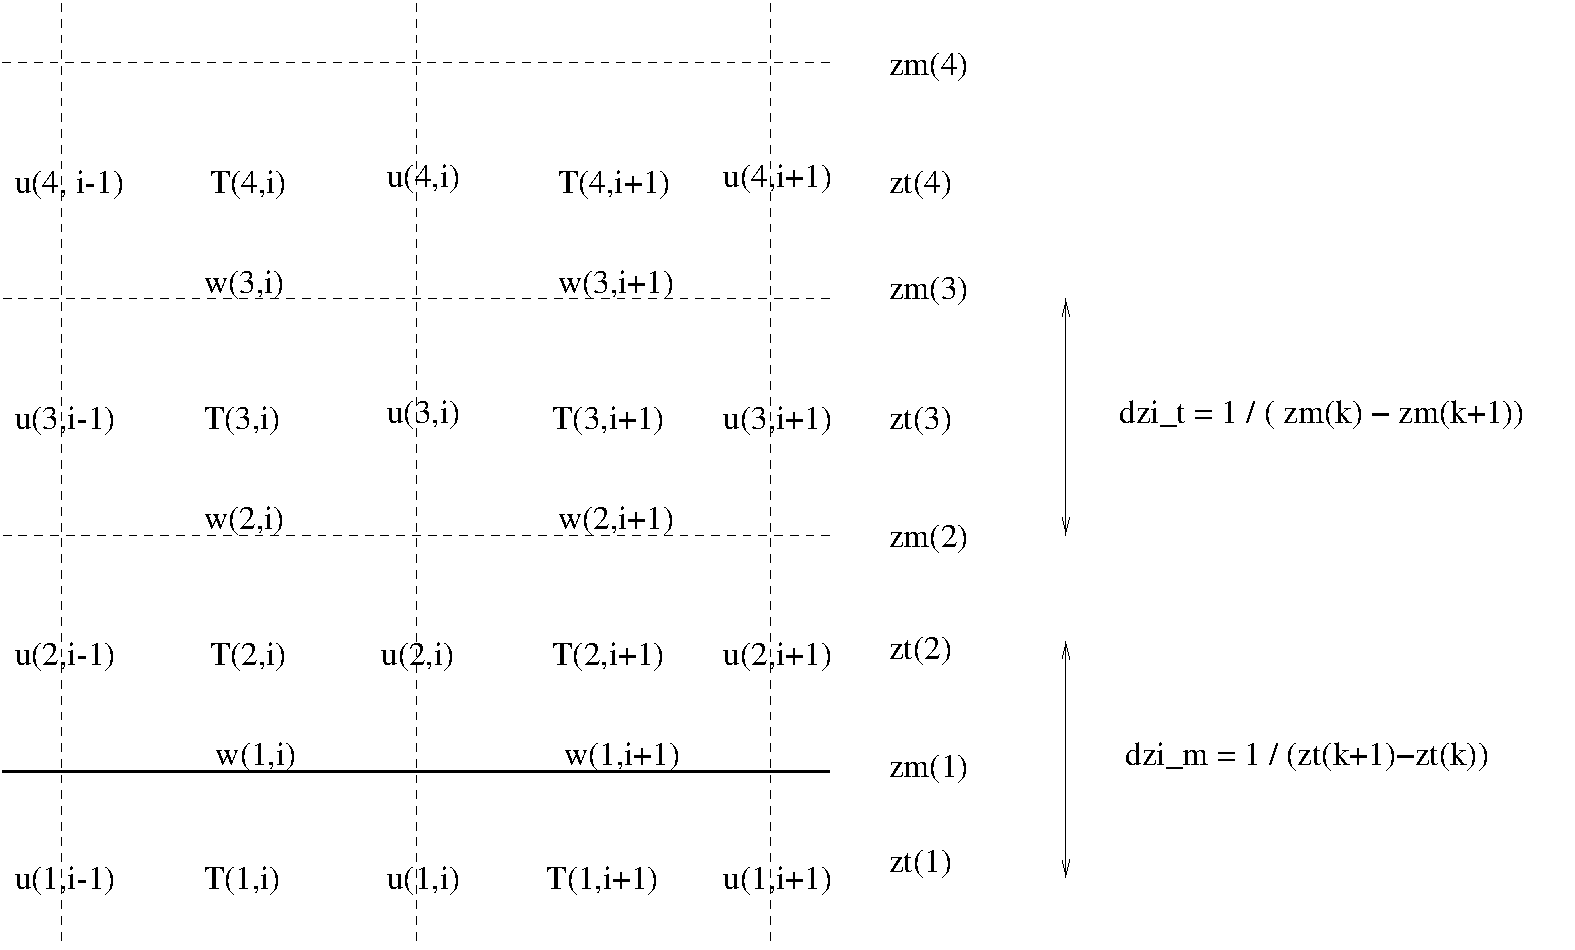
\includegraphics[height=0.5\textheight]{grid2.pdf}
\end{column}
\begin{column}{0.45\textwidth}
 \begin{itemize}
  \item The grid is staggered as a Arakawa C-grid
  \item Pressure and scalars are defined at cell center
  \item The velocities are defined at the cell faces to avoid decoupling between pressure and velocity
  \item The upper/right cell face has the same index as the cell center
 \end{itemize}

\end{column}

\end{columns}
\end{frame}


\author{Thijs Heus}
\lecture[Statistics]{Statistics and output}{statistics}
\begin{frame}[allowframebreaks]{Output files}
 \begin{itemize}
  \item Restart files \code{*.rst} only for internal model use. Output every \code{frqhis} seconds
  \item 3D output files \code{name.nc}: 3D output of the main quantities. Output done every \code{frqanl} seconds. Bulky!
  \item 2D Crosssections \code{name.out.cross*nc}: Crosssections of the data in th xy, xz, yz planes, as well as 2D integrated quantities like Liquid Water Path. Output done every \code{frqcross} seconds, governed by \code{lcross}, \code{lxy}, \code{lxz}, \code{lyz}
  \item 1D Profiles \code{name.ps*nc}. Profiles as a function of height. Output every \code{savg\_intvl}, sampling every \code{ssam\_intvl}. Need to be post processed for MPI runs.
  \item Timeseries \code{name.ts.*nc}. Domain averaged surface values, liquid water paths, cloud fraction etc. Output and sampling done every \code{ssam\_intvl}. Needs to be post processed for MPI runs.
 \end{itemize}
\end{frame}
\begin{frame}[allowframebreaks]{Statistics and output}
\mylineno=0\begin{longtable}{p{0.15\linewidth}p{0.15\linewidth}p{0.6\linewidth}}
\alert{Variable} &\alert{Default} & \tblnewline 
\endhead
outflg    &  true   &  output flag (true/false) \tblnewline
lsync & false &  Synchronize the crosssection output (true/false)\tblnewline
frqhis    &  9000 s &  history write interval \tblnewline
frqanl    &  3600 s &  analysis write interval  \tblnewline
slcflg    &  false  &  write slice output (true/false) \tblnewline 
istpfl    &  1 &  print interval for timestep info \tblnewline
ssam\_intvl&    30 s  &  statistics sampling interval\tblnewline
savg\_intvl&  1800 s    &  statistics averaging interval \tblnewline
lcross & false &  Crosssection output (true/false)\tblnewline
frqcross    &  3600 s &  crosssection write interval  \tblnewline
lxy & false &  Crosssection output in xy plane (true/false)\tblnewline
zcross & 0 &  Crosssection location of xy plane (true/false)\tblnewline
lxz & false &  Crosssection output in xz plane (true/false)\tblnewline
ycross & 0 &  Crosssection location of xy plane (true/false)\tblnewline
lyz & false &  Crosssection output in yz plane (true/false)\tblnewline
xcross & 0 &  Crosssection location of xy plane (true/false)\tblnewline
lwaterbudget & false &  Crosssection of (costly) waterbudget (true/false)\tblnewline
\end{longtable}
\end{frame}

\begin{frame}{Timeseries}
\begin{itemize}
 \item  Postprocessing to make 1 file out of all the files per processor
 \item Build tool in \code{uclales/misc/synthesis}: 
 \item \code{ifort reducets.f90 -o reducets \textasciigrave /path/to/netcdflib/bin/nc-config --fflags --flibs \textasciigrave }
 \item \alert{NOTE: The quotation marks are accent graves (Under the tilde at a US International keyboard}
  \item Use it to gather your timeseries statistics with:
\code{reducets name nx ny}
\begin{itemize}
 \item \code{name} is the \emph{stem} of the filename (so everything before \code{.ts.00....}
 \item  \code{nx} is the number of processes in the x-direction
 \item \code{ny} is the number of processes in the y-direction
\end{itemize}
\end{itemize}
\end{frame}

\begin{frame}{Profiles}
\begin{itemize}
 \item  Postprocessing to make 1 file out of all the files per processor
 \item Build tool in \code{uclales/misc/synthesis}: 
 \item \code{ifort reduceps.f90 -o reduceps \textasciigrave /path/to/netcdflib/bin/nc-config --fflags --flibs \textasciigrave }
 \item \alert{NOTE: The quotation marks are accent graves (Under the tilde at a US International keyboard}
  \item Use it to gather your profile statistics with: \code{reduceps name nx ny}
\begin{itemize}
 \item \code{name} is the \emph{stem} of the filename (so everything before \code{.ps.00....}
 \item  \code{nx} is the number of processes in the x-direction
 \item \code{ny} is the number of processes in the y-direction
\end{itemize}
\end{itemize}
\end{frame}
\begin{frame}{Adding to Profiles and Timeseries}
 \begin{itemize}
  \item Both profiles and timeseries are written from \code{ncio.f90} and \code{stat.f90}
  \item They are known to change over time. 
 \end{itemize}

\end{frame}

\begin{frame}{Plot}
 \begin{itemize}
  \item You're completely free to do what you want :)
  \item Depending on who you are and what you want for a plot, you could use NCL, Matlab, Python, Ferret, NCView,...
  \item We'd like to build up a tools database, so feel even more free to submit scripts over git
  \item As a starter, copy the 2 \code{plotfld.*} scripts from \code{uclales/misc/analysis/}
  \item Explore \code{plotfld.csh}, and put in the right variable names and time frame.
  \item Run it!
  \item Output sits in two pdf files \code{t1.pdf} and \code{p1.pdf}
 \end{itemize}
\end{frame}

\begin{frame}{Crosssections}
\begin{itemize}
 \item Postprocessing to make 1 file out of all the files per processor:
\item \code{cdo gather name.out.cross*nc name.out.cross.nc}
\item Watch the file quickly with (for instance) \code{ncview}
\end{itemize}

 

\end{frame}



\author{Thijs Heus}
\lecture[Dynamics]{Advection, diffusion and subgrid}{dynamics}
% \section[Equations]{The LES Equations}
\begin{frame}[label=equations]{The LES Equations}
\framesubtitle<4>{Advection}
\framesubtitle<5>{Diffusion}
\framesubtitle<6>{Pressure}
\framesubtitle<7>{Other forces}
Solving velocity $\bar{u}_j$ and scalars $\bar{\phi}$ includes \memph<4>{Advection}, \memph<5>{Diffusion}, \memph<6>{Pressure} and \memph<7>{other forces and sources}.
\begin{align*}
\frac{\partial \bar{u}_i}{\partial t} & = 
&\memph<4>{- \bar{u}_j \frac{\partial \bar{u}_i}{\partial x_j} }
&\memph<6>{- c_p \Theta_0 \frac{\partial\bar{\pi}}{\partial x_i}}
&\memph<5>{+ \frac{1}{\rho_0} \frac{\partial (\rho_0 \tau_{ij})} {\partial x_j}}
&\memph<7>{ + \force{i}{} }
\\
\frac{\partial \bar{\phi}}{\partial t} & = 
&\memph<4>{ - \bar{u}_j \frac{\partial  \bar{\phi}}{\partial x_j}} 
&&\memph<5>{+ \frac{1}{\rho_0} \frac{\partial (\rho_0  \gamma_{\phi j})} {\partial x_j}}
&\memph<7>{+\source{\phi}{}}
\end{align*}
\only<2->{
Anelastic continuity $$
 \frac{\partial (\rho_0 u_i) }{\partial x_i} = 0 
$$
}
\only<3->{
Ideal gas law equation of state $$\theta_v = \theta\left[1 + (\frac{R_v}{R_d}-1)q_t - \frac{R_v}{R_d}q_l\right].$$
}
\end{frame}
\section[Time]{Timestepping}
\begin{frame}[allowframebreaks]{Timestepping}
Time stepping is based on a Runge-Kutta third order method. 

The tendencies are calculated through 3 iterations:
\begin{align*}
	\phi_*^{n} &=& \phi^{n} &+& \alpha_1 \frac{\partial \phi^{n}}{\partial t} \Delta t& \\
	\phi_{**}^{n} &=& \phi_*^{n} &+& \alpha_2 \frac{\partial \phi^{n}}{\partial t} \Delta t &+& \beta_2 \frac{\partial \phi_*^{n}}{\partial t} \Delta t \\
 	\phi^{n+1} &=& \phi_{**}^{n} &+& \alpha_3 \frac{\partial \phi_{**}^{n}}{\partial t} \Delta t &+& \beta_3 \frac{\partial \phi_*^{n}}{\partial t} \Delta t
\end{align*}
With $\alpha_i = (\frac{8}{15}, -\frac{17}{60}, \frac{3}{4})$
and $\beta_i = (0, -\frac{15}{12}, -\frac{15}{12})$.	
\pagebreak
\begin{itemize}
 \item The timestep $\Delta t$ (or \code{dt}.) in the code is variable
\item Bounded by the Courant criterion ($CFL = 0.5$)
\item Bounded by \code{dt\_long} in \code{NAMELIST}. Use it for: 
\begin{itemize}
 \item Unstabilties not in advection
 \item Unstable spin ups
 \item Circumventing bugs (but fix them later!)
\end{itemize}

\item \emph{Not} bounded by e.g. statistical timesteps. First step after $t_{samp}$ is taken for statistics; faster but slightly imprecise.
\end{itemize}
 
% % 
% The model employs a variable timestep, which is set so as to maintain
% a constant CFL maximum value bounded above by the value of the maximum
% timestep (dtlong in the NAMELIST file). If dtlong exceeds the maximum
% CFL value the actual timestep is scaled so that CFL value according
% to the new timestep is always 0.5.
\end{frame}
\section[Advection]{Advection}
\againframe<4>{equations}
\begin{frame}{Advection}

Advection can be best thought of flux through the boundaries of the cell:
\begin{align*}
 \derr{\bar{u_i}\phi_i}{x} &=& \frac{F_{i+\frac{1}{2}}-F_{i-\frac{1}{2}}}{\Delta x}
\end{align*}
 with $F_{i+\frac{1}{2}}$ the flux through the cell boundary at ${i+\frac{1}{2}}$.


\end{frame}
\begin{frame}{Advection}
\begin{center}
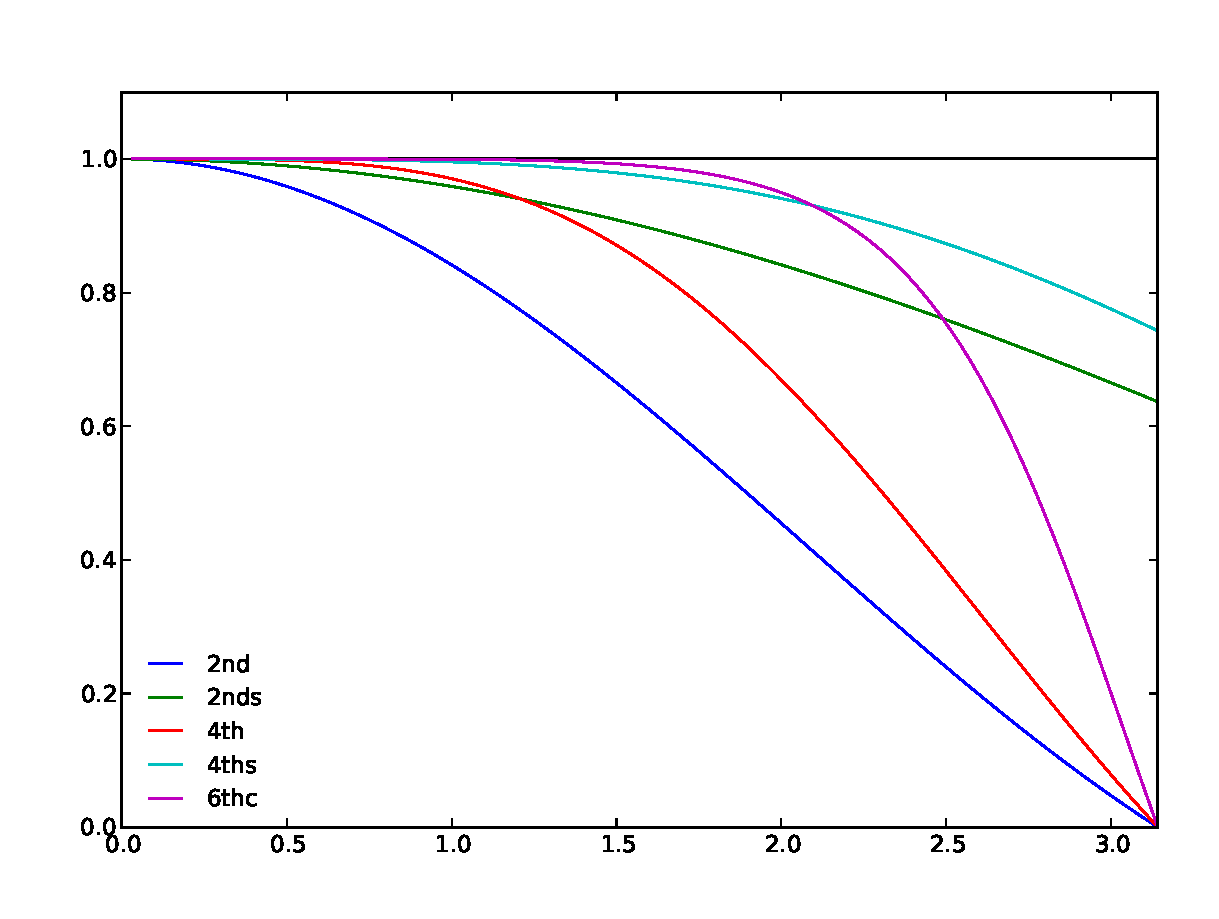
\includegraphics[height=0.7\textheight]{modkratio.pdf}       
\end{center}

\end{frame}
\begin{frame}{Advection}
\begin{center}
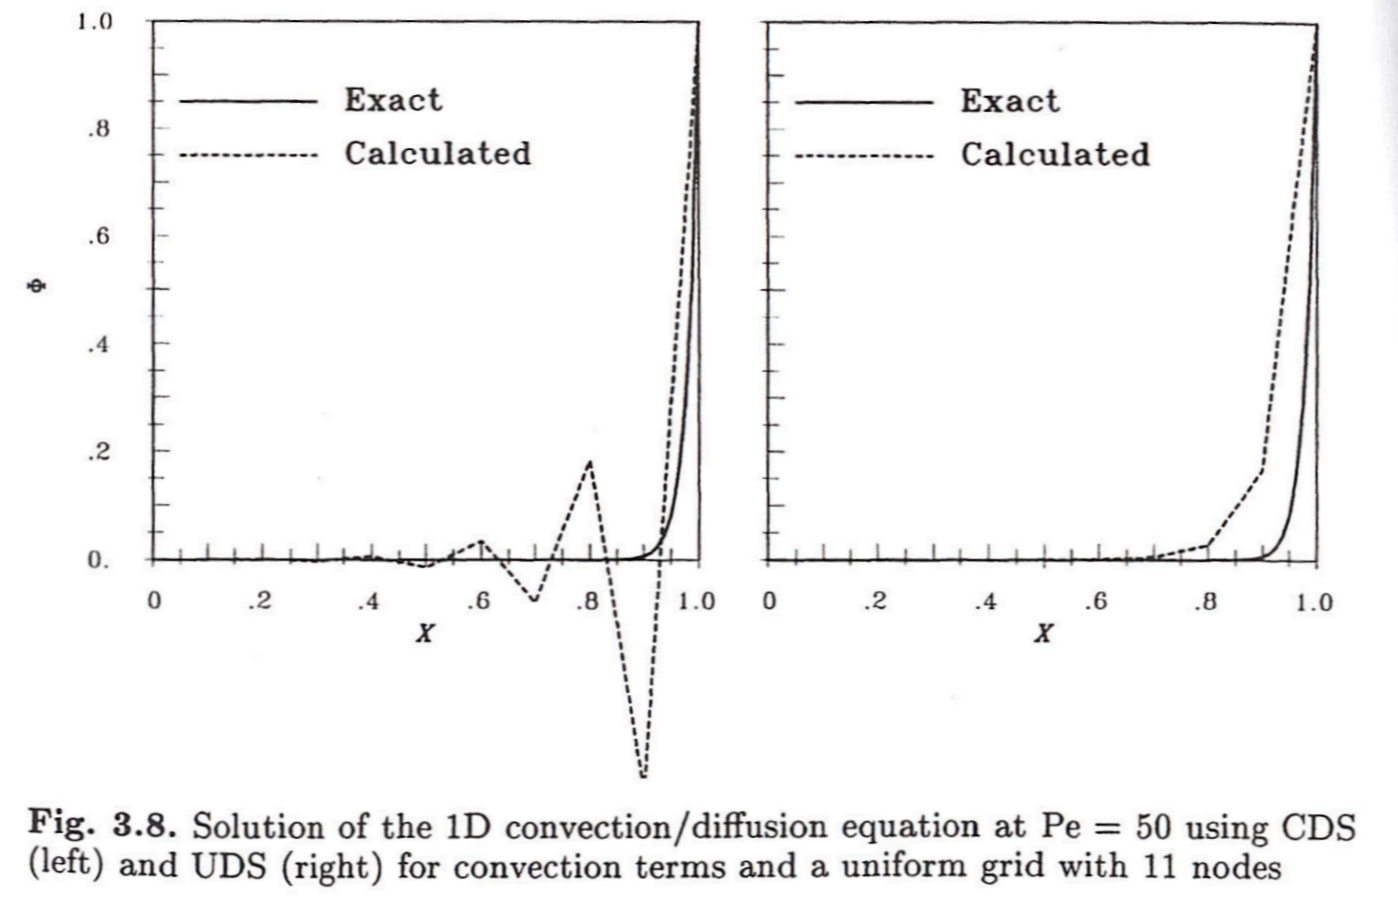
\includegraphics[height=0.7\textheight]{wiggles.png}       
\end{center}

\end{frame}

\begin{frame}{Advection}
\framesubtitle{4th order}
In UCLALES, we do 4th order Central Differencing for momentum advection, and flux-limited advection for scalars to guarantee positive values
\begin{align*}
 F^{4th}_{i+\frac{1}{2}} &=& \frac{u_{i+\frac{1}{2}}}{12} \left[-\phi_{i-1} + 7 \phi_{i} + 7 \phi_{i+1} -\phi_{i+2}\right]
\end{align*}
\pause
\begin{align*}
 F_{i+\frac{1}{2}}^{\kappa} &=& \bar{u}_{i+\frac{1}{2}} \left[\phi_{i}+\frac{1}{2}\kappa_{i+\frac{1}{2}}\left(\phi_{i}-\phi_{i-1}\right)\right]
\end{align*}
With $\kappa_{i+\frac{1}{2}} > 0 $ and a function of consecutive gradients (assuming $u_{i+\frac{1}{2}}$):
$ r = \frac{\phi_{i+1} - \phi_{i}}{\phi_{i} - \phi_{i-1}} $
\end{frame}



\begin{frame}[<+->]{Flux limiter schemes}
Depending on the setting \code{lmtr} in \code{advf.f90}, we use:
\begin{align*}
 \mathrm{\mathbf{minmod}\ } & \mathrm{min}\left(r, 1\right)  \\
 \mathrm{\mathbf{superbee}\ } & \mathrm{max}\left(\mathrm{min}\left(2 r, 1\right), \mathrm{min}\left(r, 2\right)\right)\\
 \mathrm{\mathbf{MC}\ } & \mathrm{min}(2 r,\frac{1+r}{2}, 2)  \\
 \mathrm{\mathbf{vanLeer}\ } & \frac{r + |r|}{1 + |r|}
\end{align*}
By default, it is set to MC.

Effectively, limiter schemes switch back to low order upwind schemes whenever the local gradient is to steep. 

\emph{This happens a lot in turbulent fields. This can cause so much diffusion that the SFS scheme is rendered useless}
\end{frame}

\section[Diffusion]{Diffusion}
\againframe<5>{equations}
\begin{frame}[allowframebreaks]{Diffusion}
The sub-grid fluxes $\tau_{ij}$ and $\gamma_{\phi j}$ are not known
explicitly and thus must be modeled.  This constitutes the model
closure.  The basic or default form of the closure makes use of the
Smagorinsky model, wherein
\begin{equation*}
\tau_{ij} = - \rho_0 K_mD_{ij} \quad \text{and} \quad \gamma_{\phi j}
= - \frac{K_m}{Pr} \frac{\partial \bar{\phi}} {\partial x_j},
\end{equation*}
where \[D_{ij} = \frac{\partial \bar{u}_i}{\partial x_j} +
\frac{\partial \bar{u}_j}{\partial x_i}\] is the resolved deformation,
$K_m$ is the eddy viscosity, and $Pr$ is an eddy Prandtl number.  The
Smagorinsky model calculates the eddy viscosity as
\begin{equation*}
K_m = (C_s \ell)^2 S \sqrt{1 - \frac{Ri}{Pr}} \quad \text{where} \quad
Ri =
\frac{S^2}{N^2}
\end{equation*}
and
\begin{equation*}
S^2 \equiv \frac{\partial \bar{u}_i}{\partial x_j} D_{ij} \quad
\text{and} \quad N^2 = \frac{g}{\Theta_0} \frac{\partial
\bar{\theta}_v}{\partial z}.
\end{equation*}
In the above $C_s$ is the Smagorinsky constant and takes on values
near 0.2, and
\[ \ell^{-2} = (\Delta x \Delta y \Delta z)^{-2/3} + (z\kappa/C_s)^{-2},
\]  where $\kappa=0.35$ is the von K\'arm\'an constant in the model. 
\end{frame}

\section[Pressure]{Pressure}
\againframe<6>{equations}
\begin{frame}[allowframebreaks]{Pressure(s)}
Exner function: $\bar{\pi}=(\bar{p}/p_{00})^{R_d/c_p}$ 

The anelastic approximation solves for perturbations about a
hydrostatic basic state of constant potential temperature, i.e.,
\begin{equation*}
\frac{d\pi_0}{dz} = -\frac{g}{c_p\Theta_0},
\end{equation*}
where subscript $0$ denotes a basic state value, which depend only on
$z$ ($\Theta_0$ being constant).  

For gravity, we use buoyancy deviations from the slab average (not the basic state).
For consistency, introduce a second exner $\pi_1$:

\begin{equation*}
\frac{d}{dz}(\pi_0 + \pi_1) = -\frac{g}{c_p\bar{\theta_v}},
\end{equation*}
\end{frame}
\begin{frame}{Calculating Pressure I}
Start with continuity:
\[
  \frac{\partial (\rho_0 u_i) }{\partial x_i} = 0 
\]
\pause
And the momentum equation:
\[
\frac{\partial \bar{u}_i}{\partial t}  = 
{- \bar{u}_j \frac{\partial \bar{u}_i}{\partial x_j} }
{- c_p \Theta_0 \frac{\partial\bar{\pi}}{\partial x_i}}
{+ \frac{1}{\rho_0} \frac{\partial (\rho_0 \tau_{ij})} {\partial x_j}}
{ + \force{i}{} } 
\]
\pause
Fill them in in each other:
\[
\derr{}{x_i}\left(\rho_0\frac{\partial \bar{u}_i}{\partial t}\right)   =\derr{}{x_i}\left[
- \rho_0\bar{u}_j \frac{\partial \bar{u}_i}{\partial x_j} 
- \rho_0 c_p \Theta_0 \frac{\partial\bar{\pi}}{\partial x_i}
+ \frac{\partial (\rho_0 \tau_{ij})} {\partial x_j}
{ + \rho_0\force{i}{} }\right] = 0
\]
\end{frame}
\begin{frame}{Calculating Pressure II}
\[
\derr{}{x_i}\left[
- \rho_0\bar{u}_j \frac{\partial \bar{u}_i}{\partial x_j} 
- \rho_0 c_p \Theta_0 \frac{\partial\bar{\pi}}{\partial x_i}
+ \frac{\partial (\rho_0 \tau_{ij})} {\partial x_j}
{ + \rho_0\force{i}{} }\right] = 0
\]
Bring the pressure to the other side:
\[
\derr{}{x_i}\left(\rho_0{ c_p \Theta_0 \frac{\partial\bar{\pi}}{\partial x_i}}\right)   = \derr{}{x_i}\left[
- \rho_0\bar{u}_j \frac{\partial \bar{u}_i}{\partial x_j} 
+ \frac{\partial (\rho_0 \tau_{ij})} {\partial x_j}
{ + \rho_0\force{i}{} }\right] 
\]
\pause
And we end up with a Poisson equation:
\[
\derr{}{x_i}\left(\rho_0{\frac{\partial\bar{\pi}}{\partial x_i}}\right)   = \frac{1}{ c_p \Theta_0 }\derr{}{x_i}\left[
- \rho_0\bar{u}_j \frac{\partial \bar{u}_i}{\partial x_j} 
+ \frac{\partial (\rho_0 \tau_{ij})} {\partial x_j}
{ + \rho_0\force{i}{} }\right] 
\]
that can be solved efficiently (but globally!) in Fourier space.
\end{frame}

\author{Cathy Hohenegger}
\lecture[Surface]{The surface model}{surface}


{
\setbeamercolor{background canvas}{bg=}

\includepdf[pages=2-]{LEScourse_surface.pdf}
}

\author{Axel Seifert}
\lecture[Microphysics]{Microphysics and Thermodynamics}{microphysics}


{
\setbeamercolor{background canvas}{bg=}

\includepdf[pages=2-]{UCLA-LES_micro_lecture.pdf}
}


\author{Bjorn Stevens}
\lecture[Radiation]{Radiation}{radiation}

% \author{Thijs Heus}
\lecture[Forcings]{Other Forces and Sources}{other}
\begin{frame}{Other Forces and Sources}
\begin{itemize}
 \item Gravity
 \item Coriolis and Geostrophy
 \item Sponge
 \item Nudge
\end{itemize}
\end{frame}

\lecture[Exercises]{Excercises}{excercises}

% \author{Thijs Heus}
% \lecture[Dry CBL]{The Dry Convective Boundary Layer}{drycbl}
\begin{frame}{The Dry Convective Boundary Layer}
\begin{itemize}
 \item Run the code with \code{uclales/misc/initfiles/namelist\_drycbl}
 \item Process the statistics with \code{reduceps} and \code{reducets}
 \item Stitch the crosssections together with \code{cdo gather} 
 \item Plot with \code{ncview}, \code{ncl}, the scripts in \code{uclales/misc/analysis}, or your program of choice
\end{itemize}
\end{frame}

\begin{frame}[allowframebreaks]{Questions}
 \begin{itemize}
  \item What are the profiles of the 3 velocity components? Do you understand that?
  \item There are 3 different ways of defining the boundary layer height \code{zi}:
\begin{itemize}
 \item The maximum gradient in $\theta_l$
 \item The maximum variance in $\theta_l$
 \item The minimum buoyancy flux
\end{itemize}
 \item What are the differences? 
 \item The encroachment rate is equal to: \[z_{enc}(t) = \sqrt{\frac{2 F t}{\Gamma}}\] with $F$ the surface heat flux and $\Gamma$ the temperature lapse rate. How does $z_i$ compare with $z_{enc}$? What is the difference?

 \item Look at the variances: \code{u2, w2, t2}. What do they look like? What is/is not with what you expect from Boundary Layer theory?
 \item Look at the vertical flux profiles, and in particular \code{tot\_tw} and \code{sfs\_tw}. 
 \item Finally, compare the advective tendency (\code{adv\_u}) with the diffusion(\code{dff\_u}). What do you notice? Would you say that the LES is well resolved? Where / why (not)?
\pagebreak
 \item \textbf{Optional, to be done after the Statistics class:} It would be very useful to have conditional sampling of the thermal updrafts. Unfortunately, they are not in the \code{.ps} file at the moment. As a (lengthier) exercise, we are going to do that here.
 \item Open the files \code{ncio.f90} and \code{stat.f90}. First, have a look at \code{stat.f90}
 \item The name of a \code{ps} variable is defined in \code{s2} from line 52 on. This includes the \code{cs2} variables for buoyant cloud conditional sampling. Append \code{cs3} variables for (at least) $w$ and $tv$ at the end of the array. Raise \code{nvar2} at l.33 accordingly.
 \item Make sure you know the number of your new variables.
 \item The conditional sampling for cloud water is done in subroutine \code{accum\_lvl2} between lines 604 and 658. Look at those in depth.
 \item The function \code{get\_avg} creates an average over the 2 horizontal direction out of a 3D array.
 \item The function \code{get\_csum} creates a conditional sum over an array, on places where  the final array is 1
 \item Use these lines for a conditional sampling of dry thermals. Put it in subroutine \code{accum\_lvl1}
 \item In \code{ncio.f90} the variable output names, longnames and units are provided. Use the code from line 989 on as an example to add your variables.
 \item That should be all: Try and compile. Now it gets time to debug.
 \end{itemize}

\end{frame}


\author{Thijs Heus}
% \lecture[Cumulus]{BOMEX Shallow Cumulus}{cumulus}
\begin{frame}{BOMEX Shallow Cumulus}
\begin{itemize}
 \item Check \code{articles/siebesma2003.pdf} for the initial settings of BOMEX
 \item Build a \code{NAMELIST} based on it. Hint: the \code{RICO} Namelist should be a good starting point
 \item Run the run, postprocess like the Dry CBL run
 \item If successful, commit your NAMELIST to git
 \item Rerun your run with a different name, but with \code{level=3} for microphysics in the NAMELIST
\end{itemize}
\end{frame}

\begin{frame}[allowframebreaks]{Questions}
 \begin{itemize}
  \item Plot the cloud fraction and the cloud cover. What is the difference between the two?
  \item What are cloud base and cloud top? There are several cloud bases/tops in the \code{.ts} file. What is the difference between them? What can we (implicitly) learn about these clouds based upon these numbers?
  \item One classical way of parametrizing (shallow) cumuli in large scale models, is to model the transport through the cloud layer with a mass flux approach. If necessary, read up on it in \code{siebesma1995.pdf}. They found that entrainment and detrainment rates in the large scale models were off by an order of magnitude.
  \item Try and reproduce figures 6 and on from that study using the output of the \code{.ps} file. \code{\_cs1} is the conditional sampling over the cloud. \code{\_cs2} is the conditional sampling for the buoyant part of the cloud.
  \item BOMEX was an intercomparison case of non-precipitating cumulus clouds. Is the non-precipitating really true, or just because of a lack of microphysical models a decade ago?
  \item  If precipitation is present, does it matter?
 \end{itemize}
\end{frame}
 
% \author{Thijs Heus}
% \lecture[Stratocumulus]{DYCOMS RF02}{stratocumulus}
\begin{frame}{DYCOMS RF02 Stratocumulus}
 \begin{itemize}
  \item The Dycoms Stratocumulus case is described in \code{ackerman2009.pdf}
  \item Done with $70 cm^{-3}$ CCN and prescribed radiation.
  \item Is the cloud layer sensitive to these kind of choices?
  \item The autoconversion rate can be switched to the Khairoutdinov/Kogan scheme (optimized for Stratocumulus) or Seifert Beheng (more general). Any difference?
  \item Compare with the results from the paper
 \end{itemize}

\end{frame}



\end{document}
